\documentclass[a4paper,11pt]{article}
\usepackage[UKenglish]{babel}
\usepackage{graphicx}
\usepackage{courier}
\usepackage{color}
\usepackage{array}
\usepackage{pstricks}
\usepackage{parskip}
\usepackage[bottom]{footmisc}
\usepackage{fancyhdr}
% the hyperref package must always be the last package to be included
\usepackage[pdftex,
            pdfusetitle,
            pdfsubject={User's Manual for dastaZ80 homebrew computer},
            pdfkeywords={Z80, homebrew computer, Operating System, OS}
        ]{hyperref}

\hypersetup{
    colorlinks = true,
    linkcolor = blue,
    anchorcolor = blue,
    citecolor = blue,
    filecolor = blue,
    urlcolor = blue
}

\setlength\parindent{0pt}

\begin{document}
    \pagestyle{empty}
    % ==========================================================================
    % Cover page
    % ==========================================================================
    \begin{pspicture}(8.5,11)
        \rput[b](3.5,8){
            \parbox{5in}{
                \begin{flushright}
                    \Huge\bfseries\sffamily dastaZ80 Mark II\\ User's Manual
                \end{flushright}
            }
        }
        \uput[0](0,0){\color{blue}\rule{5in}{0.5ex}}
    \end{pspicture}
    \title{dastaZ80 User's Manual}
    \author{David Asta}
    \date{7 September 2022}

    \pagebreak
    % ==========================================================================
    % Header & Footer
    % ==========================================================================
    \pagestyle{fancy}
    \fancyhf{}
    \fancyhead[R]{dastaZ80 Mark II User's Manual}
    % ==========================================================================
    \section*{Disclaimer}
    % ==========================================================================
    The products described in this manual are intended for educational purposes,
    and should not be used for controlling any machinery, critical component in
    life support devices or any system in which failure could result in personal
    injury if any of the described here products fail.
    
    These products are subject to continuous development and improvement. All
    information of a technical nature and particulars of the products and its
    use are given by the author in good faith. However, it is acknowledged that
    there may be errors or omissions in this manual. Therefore, the author
    cannot accept any liability for any loss or damage arising from the use of
    any information or particulars in this manual.

    % ==========================================================================
    \section*{Licenses}
    % ==========================================================================
    \small
    \textbf{Hardware} is licensed under the \textbf{Creative Commons
    Attribution-ShareAlike 4.0 International License}
    
    \hspace{1cm}http://creativecommons.org/licenses/by-sa/4.0/
    
    \textbf{Software} is licensed under \textbf{The MIT License}
    
    \hspace{1cm}https://opensource.org/licenses/MIT
    
    \textbf{Documentation} is licensed under the \textbf{Creative Commons
    Attribution-ShareAlike 4.0 International License}
    
    \hspace{1cm}http://creativecommons.org/licenses/by-sa/4.0/

    \normalsize

    \hrulefill

    \textcopyright 2022 David Asta

    \pagebreak
    % ==========================================================================
    \section*{Document Conventions}
    % ==========================================================================
    The following conventions are used in this manual:

    \begin{center}
        \begin{tabular}{c m{9cm}}
            \hline
            MUST & MUST denotes that the definition is and absolute
            requirement.\\
            \hline
            SHOULD & SHOULD denotes that it is recommended, but that there may
            exist valid reasons to ignore it.\\
            \hline
            \textbf{DEVICE} & Device names are displayed in bold all upper case 
            letters, and refer to hardware devices.\\
            \hline
            \textbf{command} & Operating System command keywords are displayed 
            in bold all lower case letters.\\
            \hline
            \textit{$<$text$>$} & Angle brackets enclose variable information 
            that you MUST supply. In place of \textit{$<$text$>$}, substitute 
            the value desired. Do not enter the angle brackets when entering the
            value.\\
            \hline
            \textit{$[$text$]$} & Square brackets enclose variable information
            that you COULD supply. They are optional. In place of $[$text$]$,
            substitute the value desired. Do not enter the square brackets when
            entering the value.\\
            \hline
            \texttt{Courier} & Text appearing in the \texttt{Courier} font 
            represents information that you type in via the keyboard.\\
            \hline
            0x14B0 & Numbers prefixed by 0x indicate an Hexadecimal value.
            Unless specified, memory addresses are always expressed in
            Hexadecimal.\\
            \hline
            \textit{Return} & Refers to the key Return in the keyboard.\\
            \hline
        \end{tabular}
    \end{center}

    The SD card is referred as \textbf{DISK}.

    The Floppy Disk Drive is referred as \textbf{DISK} or as \textbf{FDD}.

    The 80 column text VGA output is referred as \textbf{CONSOLE} or as
    \textbf{High Resolution Display}.

    The 40 column graphics Composite Video output is referred as \textbf{Low
    Resolution Display}.
    
    The Operating System may be referred as DZOS, dzOS or simply OS.

    \textbf{MEMORY} refers to both \textbf{ROM} and \textbf{RAM}.

    Memory used by the \textbf{Low Resolution Display} is referred as
    \textbf{VRAM} (Video RAM).
    
    \pagebreak
    % ==========================================================================
    \section*{Related Documentation}
    % ==========================================================================
    \begin{itemize}
        \item dastaZ80 User's Manual\cite{dastaz80userman}
        \item dastaZ80 Technical Reference Manual\cite{dastaz80techman}
        \item dzOS Github Repository\cite{dastaZ80github}
        \item Software for dzOS Github Repository\cite{dastaZ80githubsoft}
    \end{itemize}

    \pagebreak
    % ==========================================================================
    \tableofcontents
    % ==========================================================================

    \pagebreak
    % ==========================================================================
    % Header & Footer
    % ==========================================================================
    \pagestyle{fancy}
    \fancyhf{}
    \fancyhead[R]{dastaZ80 Mark II User's Manual}
    \fancyfoot[R]{\thepage}
    \setcounter{page}{1}
    % ==========================================================================
    \section{Introduction}
    % ==========================================================================
    The dastaZ80 is a homebrew computer designed and built following the style
    of the 8-bit computers of the 80s that I used on those days: Amstrad CPC,
    Commodore 64 and MSX). The name comes from “d”avid “asta” (my name) and 
    “Z80” (the CPU used).

    The idea behind the making of this computer came from an initial wish of
    writing an operating system (OS) for an 8-bit machine. Not comfortable with
    writing an OS for an already existing computer like an Amstrad CPC, C64,
    MSX, etc., due to the complexity of its hardware, I decided to built my own
    8-bit computer from scratch, so that I could fully understand the hardware
    and also influence the design.

    The OS written by me for this computer is called \textit{DZOS}, from 
    dastaZ80 OS. Sometimes I spell it as \textit{dzOS}. Haven’t made my mind 
    yet.

    This manual describes the usage of DZOS running on a dastaZ80 computer.
    Nevertheless, due to its design principles DZOS is portable to other 8-bit
    machines and hence mostly everything described here is applicable to DZOS
    running on other computers.
    
    \pagebreak
    % ==========================================================================
    \section{dastaZ80 Overview}
    % ==========================================================================
    \begin{itemize}
        \item Zilog Z80 microprocessor (CPU) running at 7.3728 MHz
        \item 64 KB \textbf{MEMORY}
        \begin{itemize}
            \item 16 KB reserved for DZOS
            \item 48 KB available for the user
            \item 56 Bytes NVRAM
        \end{itemize}
        \item Storage devices
        \begin{itemize}
            \item Micro SD Card, formatted with FAT32 and containing Disk Image
            Files formatted with DZFS\footnote{DZFS (dastaZ80 File System) is a
            file system of my own design, for mass storage devices, aimed at
            simplicity.}
            \item 3.5" DD/HD Floppy Disk Drive
        \end{itemize}
        \item Dual Video output
        \begin{itemize}
            \item VGA 80 columns by 25 lines and 16 colours
            \item Composite NTSC 15 colours
        \end{itemize}
        \item Real-Time Clock
        \begin{itemize}
            \item DS3231 RTC, provides valid until the year 2100 leap year
            compensation
        \end{itemize}
        \item Keyboard
        \begin{itemize}
            \item Acorn Archimedes A3010 keyboard. 102 keys with 12 function
            keys, cursor keys and numeric pad
        \end{itemize}
        \item Case
        \begin{itemize}
            \item Repurposed Acorn Archimedes A3010 case with keyboard
        \end{itemize}
        \item Expansion ports
        \begin{itemize}
            \item 2x20 pin male header. Exposes all CPU signals
        \end{itemize}
    \end{itemize}

    \pagebreak
    % ==========================================================================
    \section{Setting up the system}
    % ==========================================================================
    You will only need:

    \begin{itemize}
        \item the dastaZ80 computer.
        \item A 5 Volts (4 Amp) power supply with a female 2.1mm barrel-style DC
        connector (positive polarity).
        \item A Micro SD card.
        \item A monitor with VGA input.
        \item A monitor with NTSC Composite input.
        \item A 3.5mm jack to 3 RCA Audio/Video cable\footnote{This is the same
        cable used on the Raspberry Pi for Composite output}.
        \item A LIR2032 Li-Ion Rechargeable 3.6V Battery Button Cell
    \end{itemize}

    Steps:

    \begin{enumerate}
        \item Insert the battery LIR2032 in the battery holder. Positive goes up.
        \item On a modern PC, format the SD card with FAT32.
        \item Create a file of 33 MB on the SD card. For example using Linux 
        terminal:  \texttt{fallocate -l \$((33*1024*1024)) dastaZ80.img}
        \item Create a file named \textit{\_disks.cfg} in the root of the SD card,
        and add two lines to it:
        \begin{itemize}
            \item dastaZ80.img
            \item \#
        \end{itemize}
        \item Introduce the SD card in the SD card slot at the back of the
        computer case. This procedure MUST be performed with the computer
        switched off.
        \item Connect the VGA cable from the monitor to the VGA connector at the
        back of the computer case. This procedure SHOULD be performed with the
        computer unplugged.
        \item Connect the jack of the Audio/Video cable to the A/V connector at
        the back of the computer case. This procedure SHOULD be performed with
        the computer unplugged.
        \item Connect the female power supply connector to the male connector at
        the back of the case.
    \end{enumerate}

    That’s really it. Switch the computer on, with the power switch, and you
    should see text on your monitor. DZOS is ready to use.

    % ==========================================================================
    \subsection{Dual Video Output}
    % ==========================================================================

    The dastaZ80 has two simultaneous video outputs: VGA and Composite.

    The VGA output, called \textit{High Resolution}, is the default output for
    the Operating System. As it provides 80 columns, it is ideal for
    applications.

    The Composite output, called \textit{Low Resolution}, can only provide 40
    columns in Text Mode and 32 in Graphics Modes\footnote{This is a limitation
    imposed by the Video Display Controller used, a Texas Instruments TMS9918A.},
    making it less ideal for applications. But in contrast to the VGA output, it
    offers graphics and hardware sprites, so it makes it more suitable for video
    games and graphics output from applications.

    \pagebreak
    % ==========================================================================
    \section{Operating System (OS)}
    % ==========================================================================
    dzOS (or DZOS) is a single-user single-task ROM-based operating system (OS)
    for the 8-bit homebrew computer dastaZ80. It is heavily influenced by ideas
    and paradigms coming from Digital Research, Inc. CP/M, so some concepts may
    sound familiar to those who had used this operating system.

    The user communicates with the OS via a keyboard and a screen connected
    directly to the computer.

    The main job of dzOS is to allow the user to run programs, one at a time and
    communicate with the different peripherals (or devices, as referred in this
    manual). The user types in a command and the operating system checks what to
    do with the command received, to execute a set of instructions.

    Other tasks of dzOS are: handling disk files via its file system (DZFS),
    getting user input from the keyboard, writing messages on the screen and
    receiving/sending data through the serial port.

    dzOS consists of three parts:
    \begin{itemize}
        \item The \textbf{BIOS}, that provides functions for controlling the
        hardware.
        \item The \textbf{Kernel}, which provides general functions for
        everything that is not hardware dependent.
        \item The Command-Line Interface (\textbf{CLI}), that provides commands
        for the user to talk to the Kernel and the BIOS.
    \end{itemize}

    The Kernel and the CLI are hardware independent and will work on other Z80
    based computers. Therefore, by adapting the BIOS code, dzOS can easily be
    ported to other Z80 systems.

    % ==========================================================================
    \subsection{dastaZ80 File System (DZFS)}
    % ==========================================================================
    A file system manages access to the data stored in a storage medium, a
    SD card in the case of dastaZ80, and allows the OS to load and save data in
    the SD card. From now on, referred as \textbf{DISK}.

    DZFS is my first time designing a file system and for this reason I kept it
    very simple.

    It uses Logical Block Addressing (LBA) for accessing the data on the
    \textbf{DISK}, and an allocation table system based in blocks of sectors.
    The allocation table is called Block Allocation Table (BAT).

    Without entering into much details, bytes in the \textbf{DISK} are organised
    as Sectors, and Sectors are grouped into Blocks. Each Sector is 512 bytes
    long and each Block holds 64 Sectors. Therefore, a Block is 32,768 bytes
    long (64 * 512).

    As the free RAM of dastaZ80 is about 48 KB, it makes no sense to have files
    bigger than that, as it would not fit into \textbf{MEMORY}. Therefore, I
    have decided that each Block can store only a single file.

    % ==========================================================================
    \subsubsection{DZFS limitations}
    % ==========================================================================
    The current version of the DZFS implementation (DZFSV1) have the following
    limitations:

    \begin{itemize}
        \item No support for directories. All files are presented at the same
        level.
        \item Filenames:
        \begin{itemize}
            \item Are case sensitive.
            \item Can be maximum 14 characters long.
            \item Can only contain alphabetical (A to Z) and numerical (0 to 9)
            letters.
            \item Cannot start with a number.
            \item No support for extensions. But there is a separate field for
            File Type.
        \end{itemize}
        \item Maximum size for a file is 32,768 bytes.
    \end{itemize}
        
    \pagebreak
    % ==========================================================================
    \subsection{The Command Prompt}
    % ==========================================================================
    When you switch on the computer, the \textbf{Low Resolution Display} shows
    the computer logo:

    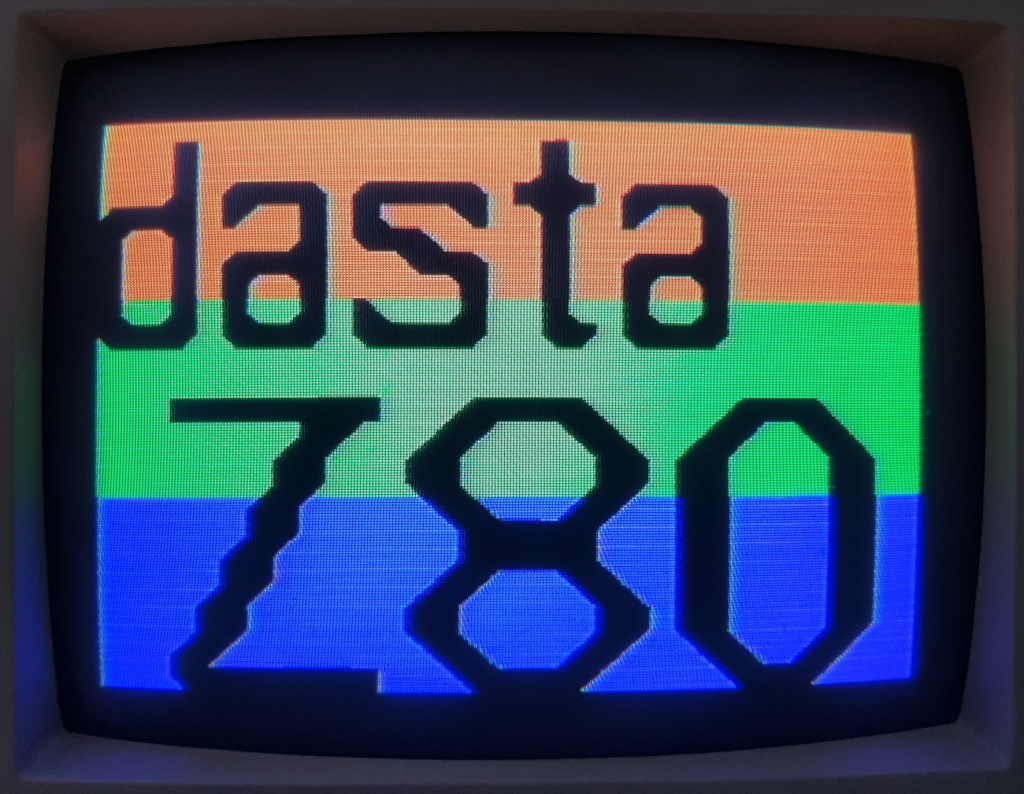
\includegraphics[scale=0.2]{dastaZ80logoOnVDP.png}

    and the \textbf{High Resolution Display}, shows some information on the
    screen:

    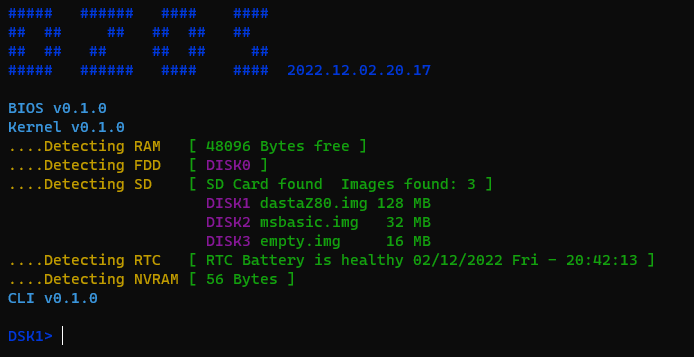
\includegraphics[scale=0.7]{dzOS.png}

    This information tells you about the release version of DZOS (2022.07.19.13
    in the screenshot). The BIOS, Kernel and CLI versions, and the detection of
    the different devices used by the computer. It also tells about whichs 
    \textbf{DISK}s are available.

    After that information,you will see the \textit{command prompt}. It starts
    with the letters \textit{DSK} (short for DISK) and a number, followed by the
    symbol $>$

    The number indicates which \textbf{DISK} is currently used for \textbf{DISK}
    operations.

    In other words, if you see \textit{DSK0}, it means that the Floppy Disk Drive
    (\textbf{FDD}) is selected. Entering commands like \textit{cat},
    \textit{diskinfo}, \textit{load}, etc., will instruct the computer to do it
    on the \textbf{FDD}.

    \pagebreak
    % ==========================================================================
    \section{OS Commands}
    % ==========================================================================
    There are a number of commands included in the operating system. These
    commands are stored in \textbf{MEMORY} at boot time, and therefore can be
    called at any time from the command prompt.

    Some commands may have mandatory and/or optional parameters. These
    parameters MUST be entered in the order listed. Interchanging the order of
    parameters will result on undesired behaviour.

    Parameters can be separated either by a comma or a space. For clarity, in
    this document all parameters are separated by a comma.

    % ==========================================================================
    \subsection{General Commands}\label{gencmds}
    % ==========================================================================
        % ======================================================================
        \subsubsection{{\color{blue}help}}
        % ======================================================================
        Shows a list of the most important commands available for the user.
        For a complete list of commands, refer always to this manual.

        \hspace{1.9cm}\textbf{$>$ help}

        \textbf{Parameters}: None

        % ======================================================================
        \subsubsection{{\color{blue}peek}}
        % ======================================================================
        Prints the value of the byte stored at a specified \textbf{MEMORY}
        address.

        \hspace{1.9cm}\textbf{$>$ peek \textit{$<$address$>$}}

        \textbf{Parameters}:

        \hspace{1cm}\textbf{\textit{address}}: address where the user wants
        to get the value from.

        \textbf{Example}: \texttt{$>$ peek 41A0}

        Will print (in hexadecimal) whatever byte is at location 0x41A0.

        % ======================================================================
        \subsubsection{{\color{blue}poke}}
        % ======================================================================
        Changes the value of the byte stored at a specified \textbf{MEMORY}
        address.

        \hspace{1.9cm}\textbf{$>$ poke \textit{$<$address$>$,$<$value$>$}}

        \textbf{Parameters}:

        \hspace{1cm}\textbf{\textit{address}}: address where the user wants
        to change a value.
        
        \hspace{1cm}\textbf{\textit{value}}: new value (in Hexadecimal notation)
        to be stored at \textit{address}.

        \textbf{Example}: \texttt{$>$ poke 41A0,2D}

        Will overwrite the contents of the address 0x41A0 with the value
        0x2D.

        % ======================================================================
        \subsubsection{{\color{blue}autopoke}}
        % ======================================================================
        Allows the user to enter a series of values to be stored at the
        starting address and its consecutive addresses. Think of it like a
        way to do poke but without having to enter the \textbf{MEMORY}
        address each time.

        After entering the command, a different command prompt, denoted by
        the symbol \$, will be displayed.

        Values are entered one by one after the symbol \$. Pressing 
        \textit{Return} with no value will end the command.

        \hspace{1.9cm}\textbf{$>$ autopoke \textit{$<$address$>$}}

        \textbf{Parameters}:

        \hspace{1cm}\textbf{\textit{address}}: address where the user wants
        to start changing values.

        \textbf{Example}: \texttt{$>$ autopoke 41A0}

        Will overwrite the contents of the address 0x41A0 with the first
        value entered by the user at the \$ prompt. Next value entered will
        overwrite the contents of the address 0x41A1, next 0x41A2, and so on
        until the end of the command.

        % ======================================================================
        \subsubsection{{\color{blue}reset}}
        % ======================================================================
        Performs a reset. It has the same effect as pressing the
        \textbf{RESET} button at the side of the computer.

        \hspace{1.9cm}\textbf{$>$ reset}

        \textbf{Parameters}: None

        % ======================================================================
        \subsubsection{{\color{blue}halt}}
        % ======================================================================
        Tells the \textbf{DISK} controller to close all files, disables
        interrupts and puts the CPU in halted state, effectively making the
        computer unusable until next power cycle (\textit{Have you tried turning
        it off and on again?}).

        SHOULD be used before switching the computer off, to ensure all
        \textbf{DISK} data has been correctly saved. MUST not be used while the
        busy light of the \textbf{DISK} is on.

        IMPORTANT: \textbf{to use the computer again, you MUST turn it off and
        on again. Do NOT just press the reset button}. Otherwise corruption of
        data will occur, because the \textbf{DISK} controller is only reset at
        power on, and not when the \textbf{RESET} button is pressed.

        \hspace{1.9cm}\textbf{$>$ halt}

        \textbf{Parameters}: None

        % ======================================================================
        \subsubsection{{\color{blue}run}}
        % ======================================================================
        There are two formats of this command:

        \textbf{run \textit{$<$address$>$}} and \textbf{run 
        \textit{$<$filename$>$}}
        
        Here the former is described. See the section \textit{\ref{dskcmds}
        DISK Commands} on page \pageref{dskcmds} for the other format.

        \hspace{1.9cm}\textbf{$>$ run \textit{$<$address$>$}}

        \textbf{Parameters}:

        \hspace{1cm}\textbf{\textit{address}}: address from where to start
        running.
        
        \textbf{Example}: \texttt{$>$ run 4420}

        Will transfer the Program Counter (PC) of the Z80 to the address
        0x4420. Therefore, the CPU will start running whatever instructions
        finds from 0x4420 and onwards. Programs run this way MUST end with a
        jump instruction (JP) to CLI prompt address, as described in the
        \textit{dastaZ80 Programmer’s Reference Guide}\cite{dastaz80progref}.
        Otherwise the user will have to reset the computer to get back to CLI.
        Not harmful but cumbersome.

        % ======================================================================
        \subsubsection{{\color{blue}crc16}}
        % ======================================================================
        Generates a CRC-16/BUYPASS1\footnote{A 16-bit cyclic redundancy
        check (CRC) based on the IBM Binary Synchronous Communications
        protocol\cite{ibmbsc} (BSC or Bisync). It uses the polynomial
        $X^{16} + X^{15} +X^2 + 1$}

        There are two formats of this command: 
        
        \textbf{crc16 \textit{$<$start\_address$>$ $<$end\_address$>$}}
        and \textbf{crc16 \textit{$<$filename$>$}} 
        
        Here the former is described. See the section \textit{\ref{dskcmds} 
        DISK Commands} on page \pageref{dskcmds} for the other format.

        \hspace{1.9cm}\textbf{$>$ crc16 \textit{$<$start\_address$>$
        $<$end\_address$>$}}
        
        \textbf{Parameters}:

        \hspace{1cm}\textbf{\textit{start\_address}}: first address from
        where the bytes to calculate the CRC will be read.

        \hspace{1cm}\textbf{\textit{end\_address}}: last address from where
        the bytes to calculate the CRC will be read.

        \textbf{Example}: \texttt{$>$ crc16 0000,0100}

        Will calculate the CRC of all bytes in MEMORY between the two
        specified address and show it on the screen:
        
        \hspace{1cm}\texttt{CRC16:\ 0x2F25}

        % ======================================================================
        \subsubsection{{\color{blue}clrram}}
        % ======================================================================
        Fills with zeros the entire Free RAM area (i.e. from 0x4420 to
        0xFFFF).

        \hspace{1.9cm}\textbf{$>$ clrram}

        \textbf{Parameters}: None

    % ======================================================================
    \subsection{Real-Time Clock (RTC) Commands}
    % ======================================================================
        % ======================================================================
        \subsubsection{{\color{blue}date}}
        % ======================================================================
        Shows the current date and day of the week from the Real-Time Clock
        (\textbf{RTC}).

        \hspace{1.9cm}\textbf{$>$ date}

        \textbf{Parameters}: None

        Will show (will differe depending on the date on the \textbf{RTC}):

        \hspace{1cm}\texttt{Today:\ 22/11/2022 Tue}

        % ======================================================================
        \subsubsection{{\color{blue}time}}
        % ======================================================================
        Shows the current time from the Real-Time Clock (\textbf{RTC}).

        \hspace{1.9cm}\textbf{$>$ time}

        \textbf{Parameters}: None

        Will show (will differe depending on the time on the \textbf{RTC}):

        \hspace{1cm}\texttt{Now:\ 16:24:36}

        % ======================================================================
        \subsubsection{{\color{blue}setdate}}
        % ======================================================================
        Changes the current date stored in the Real-Time Clock (\textbf{RTC}).

        \hspace{1.9cm}\textbf{$>$ setdate \textit{$<$yyyy$>$$<$mm$>$$<$dd$>$$<$dow$>$}}

        \textbf{Parameters}:

        \hspace{1cm}\textbf{\textit{yyyy}}: year (2 digits).

        \hspace{1cm}\textbf{\textit{mm}}: month.

        \hspace{1cm}\textbf{\textit{dd}}: day.

        \hspace{1cm}\textbf{\textit{yyyy}}: dow (Day of the Week. 1=Sunday).

        \textbf{Example}: \texttt{$>$ setdate 2211032}

        % ======================================================================
        \subsubsection{{\color{blue}settime}}
        % ======================================================================
        Changes the current time stored in the Real-Time Clock (\textbf{RTC}).

        \hspace{1.9cm}\textbf{$>$ settime \textit{$<$hh$>$$<$mm$>$$<$ss$>$}}

        \textbf{Parameters}:

        \hspace{1cm}\textbf{\textit{hh}}: hour.

        \hspace{1cm}\textbf{\textit{mm}}: minutes.

        \hspace{1cm}\textbf{\textit{ss}}: seconds.

        \textbf{Example}: \texttt{$>$ settime 185700}

    % ==========================================================================
    \subsection{Disk Commands}\label{dskcmds}
    % ==========================================================================
        % ======================================================================
        \subsubsection{{\color{blue}cat}}
        % ======================================================================
        Shows a catalogue of the files stored in the \textbf{DISK}.

        \hspace{1.9cm}\textbf{$>$ cat}

        \textbf{Parameters}: None

        \textbf{Example}: \texttt{$>$ cat}

        Will show (will differ depending on the contents of your \textbf{DISK}):

        \texttt{
        \resizebox{12cm}{!}{
            \begin{tabular}{l l l l l l}
                \multicolumn{6}{l}{Disk Catalogue}\\
                \multicolumn{6}{l}{----------------------------------------------------------------------}\\
                File & Type & Last Modified & Load Address & Attributes & Size\\
                \multicolumn{6}{l}{----------------------------------------------------------------------}\\
                HelloWorld & EXE & 12-03-2022 13:21:44 & 4420 & R SE & 38\\
                file2 & TXT & 11-05-2022 17:12:45 & 0000 & SE & 241
            \end{tabular}
        }}

        By default, deleted files are not shown in the catalogue. To show also
        deleted files do a \textit{poke 40ac, 01}. And a \textit{poke 40ac, 00}
        to hide them again.

        Deleted files are identified by a \textasciitilde symbol in the first
        character of the filename.

        \texttt{
        \resizebox{12cm}{!}{
            \begin{tabular}{l l l l l l}
                \multicolumn{6}{l}{Disk Catalogue}\\
                \multicolumn{6}{l}{----------------------------------------------------------------------}\\
                File & Type & Last Modified & Load Address & Attributes & Size\\
                \multicolumn{6}{l}{----------------------------------------------------------------------}\\
                \textasciitilde elloWorld & EXE & 12-03-2022 13:21:44 & 4420 & R SE & 38\\
                file2 & TXT & 11-05-2022 17:12:45 & 0000 & SE & 241
            \end{tabular}
        }}

        % ======================================================================
        \subsubsection{{\color{blue}erasedsk}}
        % ======================================================================
        Overwrittes all bytes of all sectors in a \textbf{DISK} in the
        \textbf{FDD}, with \texttt{0xF6} \\

        \underline{This is a destructive action} and it makes the \textbf{DISK}
        unusable to any (included dzOS) computer, as there is no file system in
        the disk after the command is completed.
        
        Before it can be used by dzOS, the command \textit{formatdsk} MUST be
        executed.

        It is recommended to only use this command in the case of wanting to
        destroy all data in a \textbf{DISK}, because \textit{formatdsk} doesn't
        actually delete any data, or to check if a Floppy Disk is faulty.
        Otherwise, the command \textit{formatdsk} SHOULD be the right command
        for normal usage of the computer.

        \hspace{1.9cm}\textbf{$>$ erasedsk}

        \textbf{Parameters}: None

        \textbf{Example}: \texttt{$>$ erasedsk}

        % ======================================================================
        \subsubsection{{\color{blue}formatdsk}}
        % ======================================================================
        Formats a \textbf{DISK} with DZFS format. \underline{This is a
        destructive action} and makes the \textbf{DISK} unsuable by any
        computers not using DZFS as their file system. It overwrites the DZFS
        \textit{Superblock} and \textit{BAT}.

        \hspace{1.9cm}\textbf{$>$ formatdsk \textit{$<$label$>$}}

        \textbf{Parameters}:

        \hspace{1cm}\textbf{\textit{label}}: a name given to the \textbf{DISK}.
        Useful for identifying different disks. It can contain any characters,
        with a maximum of 16.

        \textbf{Example}: \texttt{$>$ formatdsk mainDisk}

        Will format the SD card inserted in the SD card slot at the back of the
        computer case, having \textit{mainDisk} as disk label.

        % ======================================================================
        \subsubsection{{\color{blue}load}}
        % ======================================================================
        Loads a file from \textbf{DISK} to \textbf{RAM}.
        
        The file will be loaded in \textbf{RAM} at the address from which it was
        originally saved. This address is stored in the DZFS BAT and cannot be
        changed. 

        \hspace{1.9cm}\textbf{$>$ load \textit{$<$filename$>$}}

        \textbf{Parameters}:

        \hspace{1cm}\textbf{\textit{filename}}: the name of the file that is to
        be loaded.

        \textbf{Example}: \texttt{$>$ load HelloWorld}

        Will load the contents (bytes) of the file \textit{HelloWorld} and copy
        them into the \textbf{RAM} address from which it was originally saved.

        % ======================================================================
        \subsubsection{{\color{blue}run}}
        % ======================================================================
        There are two formats of this command:

        \textbf{run \textit{$<$address$>$}} and \textbf{run 
        \textit{$<$filename$>$}}
        
        Here the latter is described. See the section \textit{\ref{gencmds}
        General Commands} on page \pageref{gencmds} for the other format.

        \hspace{1.9cm}\textbf{$>$ run \textit{$<$filename$>$}}

        \textbf{Parameters}:

        \hspace{1cm}\textbf{\textit{filename}}: the name of the file to run.
        
        \textbf{Example}: \texttt{$>$ run HelloWorld}

        Will load the contents of the file \textit{HelloWorld} into
        \textbf{MEMORY}, and then transfer the Program Counter (PC) of the Z80
        to the address stored in the BAT entry. Therefore, the CPU will start
        running whatever instructions finds from the address and onwards.
        Programs run this way MUST end with a jump instruction (JP) to CLI
        prompt address, as described in the \textit{dastaZ80 Programmer’s
        Reference Guide}\cite{dastaz80progref}. Otherwise the user will have to
        reset the computer to get back to CLI.

        % ======================================================================
        \subsubsection{{\color{blue}rename}}
        % ======================================================================
        Changes the name of a file.

        \hspace{1.9cm}\textbf{$>$ rename \textit{$<$current\_filename$>$,
        $<$new\_filename$>$}}

        \textbf{Parameters}:

        \hspace{1cm}\textbf{\textit{current\_filename}}: the name of the file as
        existing in the \textbf{DISK} at the moment of executing this command.
        
        \hspace{1cm}\textbf{\textit{new\_filename}}: the name that the file will
        have after the command is executed.

        \textbf{Example}: \texttt{$>$ rename HelloWorld,Hello}

        Will change the name of the file \textit{HelloWorld} to \textit{Hello}.

        % ======================================================================
        \subsubsection{{\color{blue}delete}}
        % ======================================================================
        Deletes a file from the \textbf{DISK}.

        Technically is not deleting anything but just changing the first
        character of the filename to a \textasciitilde symbol, which makes it to
        not show up with the command \textit{cat}. Hence, it can be undeleted by
        simply renaming the file. But be aware, when saving new files DZFS looks
        for a free space \footnote{By free space on the \textbf{DISK} we
        understand a Block in the DZFS BAT that was never used before by a
        file.} on the \textbf{DISK}, but if it does not find any it starts
        re-using space from files marked as deleted and hence overwriting data
        on the \textbf{DISK}.

        \hspace{1.9cm}\textbf{$>$ delete \textit{$<$filename$>$}}

        \textbf{Parameters}:

        \hspace{1cm}\textbf{\textit{filename}}: the name of the file that is to
        be deleted.
        
        \textbf{Example}: \texttt{$>$ delete HelloWorld}

        Will delete the file \textit{HelloWorld}.

        % ======================================================================
        \subsubsection{{\color{blue}chgattr}}
        % ======================================================================
        Files in DZFS can have any of the following attributes:
        
        \begin{itemize}
            \item \textbf{Read Only} (R): it cannot be overwritten, renamed or
            deleted.
            \item \textbf{Hidden} (H): it does not show up in the results
            produced by the command \textit{cat}.
            \item \textbf{System} (S): this is a file used by DZOS and it MUST
            not be altered.
            \item \textbf{Executable} (E): this is an executable file and can be
            run directly with the command \textit{run $<$filename$>$}.
        \end{itemize}

        \hspace{1.9cm}\textbf{$>$ chgattr \textit{$<$filename$>$,$<$RHSE$>$}}

        \textbf{Parameters}:

        \hspace{1cm}\textbf{\textit{filename}}: the name of the file to change
        the attributes.

        \hspace{1cm}\textbf{\textit{RHSE}}: the new attributes (see list above)
        that are to be set to the specified file. Attributes are actually not
        changed but re-assigned. For example, if you have a file with attribute
        \textit{R} and specified only \textit{E}, it will change from Read Only
        to Executable. In order to keep both, you MUST specify both values,
        \textit{RE}.
        
        \textbf{Example}: \texttt{$>$ chgattr HelloWorld,RE}

        Will set the attributes of the the file \textit{HelloWorld} to Read Only
        and Executable.

        % ======================================================================
        \subsubsection{{\color{blue}save}}
        % ======================================================================
        Saves the bytes of specified \textbf{MEMORY} addresses to a new file in
        the \textbf{DISK}.

        \hspace{1.9cm}\textbf{$>$ save \textit{$<$start\_address$>$,
        $<$number\_of\_bytes$>$}}

        \textbf{Parameters}:

        \hspace{1cm}\textbf{\textit{$<$start\_address$>$}}: first address where
        the bytes that the user wants to save are located in \textbf{MEMORY}.

        \hspace{1cm}\textbf{\textit{$<$number\_of\_bytes$>$}}: total number of
        bytes, starting at \textit{start\_address} that will be saved to
        \textbf{DISK}.
        
        \textbf{Example}: \texttt{$>$ save 4420,512}

        Will create a new file, with the name entered by the user when prompted,
        with 512 bytes of the contents of \textbf{MEMORY} from 0x4420 to 0x461F.

        % ======================================================================
        \subsubsection{{\color{blue}dsk}}
        % ======================================================================
        Changes current disk for all \textbf{DISK} operations.

        \hspace{1.9cm}\textbf{$>$ dsk \textit{$<$n$>$}}

        \textbf{Parameters}:

        \hspace{1cm}\textbf{\textit{$<$n$>$}}: \textbf{DISK} number.

        \textbf{Example}: \texttt{$>$ dsk 0}

        Will change to \textbf{FDD}, and all the \textbf{DISK} operations will
        be performed in the \textbf{FDD} until the next boot or a new \textit{dsk}
        command.

        The CLI prompt changes to indicate which disk is in use.

        % ======================================================================
        \subsubsection{{\color{blue}diskinfo}}
        % ======================================================================
        Shows some information about the \textbf{DISK}.

        \hspace{1.9cm}\textbf{$>$ diskinfo}

        \textbf{Parameters}: None

        \textbf{Example}: \texttt{$>$ diskinfo}

        Will show (will differ depending on the contents of your \textbf{DISK}):

        \texttt{
        \resizebox{12cm}{!}{
            \begin{tabular}{l r l l}
                \multicolumn{4}{l}{Disk Information}\\
                & Volume .\ .\ : & dastaZ80 Main & (S/N: 352A15F2)\\
                & File System: & DZFSV1 &\\
                & Created on : & 03/10/2022 14:22:32 &\\
                & Partitions : & 01 &\\
                & Bytes per Sector: & 512 &\\
                & Sectors per Block: & 64 &
            \end{tabular}
        }}

        % ======================================================================
        \subsubsection{{\color{blue}disklist}}
        % ======================================================================
        Shows a list of all available \textbf{DISK} (\textbf{FDD} and Disk Image
        Files on the \textbf{SD}).

        \hspace{1.9cm}\textbf{$>$ disklist}

        \textbf{Parameters}: None

        \textbf{Example}: \texttt{$>$ disklist}

        Will show (will differ depending on the Disk Image Files on your
        \textbf{DISK}):

        \texttt{
        \resizebox{6cm}{!}{
            \begin{tabular}{l l l r}\\
                & DISK0 & FDD & \\
                & DISK1 & dastaZ80.img & 128 MB \\
                & DISK2 & msbasic.img   & 32 MB \\
                & DISK3 & empty.img     & 16 MB
            \end{tabular}
        }}

        \textbf{IMPORTANT}: When the list (210 bytes in total, for a maximum of
        15 Disk Image Files) is retrieved from the \textbf{ASMDC}, dzOS stores
        it at the very bottom of the RAM (\texttt{0xFF2D}). In the unlikely case
        that you may have a program loaded that uses those low bytes, after
        executing the \textit{disklist} command the program will be corrupted.

        % % ======================================================================
        % \subsubsection{{\color{blue}crc16}}
        % % ======================================================================
        % Generates a CRC-16/BUYPASS1\footnote{A 16-bit cyclic redundancy
        % check (CRC) based on the IBM Binary Synchronous Communications
        % protocol (BSC or Bisync). It uses the polynomial
        % $X^{16} + X^{15} +X^2 + 1$}

        % There are two formats of this command: 
        
        % \textbf{crc16 \textit{$<$start\_address$>$ $<$end\_address$>$}}
        % and \textbf{crc16 \textit{$<$filename$>$}} 
        
        % Here the latter is described. See the section \textit{\ref{gencmds} 
        % General Commands} on page \pageref{gencmds} for the other format.

        % \hspace{1.9cm}\textbf{$>$ crc16 \textit{$<$filename$>$}}
        
        % \textbf{Parameters}:

        % \hspace{1cm}\textbf{\textit{filename}}: the name of the file for which
        % the CRC will be calculated.

        % \textbf{Example}: \texttt{$>$ crc16 HelloWorld}

        % Will calculate the CRC of all bytes on the file and show it on the
        % screen:
        
        % \hspace{1cm}\texttt{CRC16:\ 0x3ABC}

    \pagebreak
    % ==========================================================================
    \section{Other Software}
    % ==========================================================================

    % ======================================================================
    \subsubsection{Memory Dump (memdump)}
    % ======================================================================
    This program shows the contents (bytes) of a specified range of
    \textbf{MEMORY}.

    The contents are printed as hexadecimal bytes, in groups of 16 per each line
    and with the printable ASCII value (if printable) or just a dot (if not
    printable).

    At the start of the program, the user will be asked to enter the
    \textit{Start Address} and the \textit{End Address}. In the case of leaving
    blank (i.e. just press the \textit{Return} key without entering any value),
    the program will terminate.

    Example for \textit{Start Address} = 0B40 and \textit{End Address} = 0BEF:

    \texttt{
    \resizebox{12cm}{!}{
        \begin{tabular}{l l l l l l l l l l l l l l l l l l}
                    & 00 & 01 & 02 & 03 & 04 & 05 & 06 & 07 & 08 & 09 & 0A & 0B & 0C & 0D & 0E & 0F   & \\
            \cline{2-17}
            0B40: & FF & FF & FF & FF & FF & FF & FF & FF & FF & FF & FF & FF & FF & FF & FF & 00   & ................\\
            0B50: & 21 & 3A & 0F & CD & BE & 03 & 06 & 01 & CD & 20 & 04 & CD & 4D & 0C & 21 & 56   & !:.......\ ..M.!V\\
            0B60: & 0F & CD & BE & 03 & 21 & C4 & 22 & 3E & 00 & 32 & C4 & 22 & CD & 75 & 0B & CD   & ....!.">.2.".u..\\
            0B70: & B1 & 0B & C3 & 5B & 0B & CD & C8 & 03 & FE & 20 & CA & 91 & 0B & FE & 2C & CA   & ...$[$.....\ ....,.\\
            0B80: & 91 & 0B & FE & 0D & CA & B0 & 0B & 77 & 23 & C3 & 75 & 0B & C9 & 2B & C3 & 75   & .......w\#.u..+.u\\
            0B90: & 0B & 3A & E4 & 22 & FE & 00 & CA & A4 & 0B & 3A & 04 & 23 & FE & 00 & CA & AA   & .:.".....:.\#....\\
            0BA0: & 0B & C3 & 75 & 0B & 21 & E4 & 22 & C3 & 75 & 0B & 21 & 04 & 23 & C3 & 75 & 0B   & ..u.!.".u.!.\#.u.\\
            0BB0: & C9 & 21 & C4 & 22 & 7E & FE & 00 & CA & 5B & 0B & 11 & 29 & 14 & CD & 02 & 0C   & .!."~...$[$..$)$....\\
            0BC0: & CA & 89 & 0E & 11 & 10 & 14 & CD & 02 & 0C & CA & 93 & 0E & 11 & 2C & 14 & CD   & .............,..\\
            0BD0: & 02 & 0C & CA & 55 & 0E & 11 & 25 & 14 & CD & 02 & 0C & CA & 15 & 0F & 11 & 15   & ...U..\%.........\\
            0BE0: & 14 & CD & 02 & 0C & CA & 9A & 0E & 11 & 1A & 14 & CD & 02 & 0C & CA & C7 & 0E   & ................
        \end{tabular}
    }}

    If the information reaches the bottom of the screen, a message will be shown
    to let the user decide what to do next:

    \hspace{1cm}\texttt{[SPACE] for more or another key to stop}

    % ======================================================================
    \subsubsection{Video Memory Dump (vramdump)}
    % ======================================================================
    This program shows the contents (bytes) of a specified range
    of \textbf{VRAM}.

    The contents are printed as hexadecimal bytes, in groups of 16 per each
    line.

    At the start of the program, the user will be asked to enter the
    \textit{Start Address} and the \textit{End Address}. In the case of leaving
    blank (i.e. just press the \textit{Return} key without entering any value),
    the program will terminate.

    Example for \textit{Start Address} = 0000 and \textit{End Address} = 00AF:

    \texttt{
    \resizebox{12cm}{!}{
        \begin{tabular}{l l l l l l l l l l l l l l l l l l}
                    & 00 & 01 & 02 & 03 & 04 & 05 & 06 & 07 & 08 & 09 & 0A & 0B & 0C & 0D & 0E & 0F   & \\
            \cline{2-17}
            0000: & 00 & 00 & 00 & 00 & 00 & 00 & 00 & 00 & FF & FF & FF & FF & FF & FF & FF & FF\\
            0010: & 00 & 00 & 00 & 00 & 00 & 01 & 03 & 07 & 00 & 00 & 00 & 00 & 00 & 80 & C0 & E0\\
            0020: & 07 & 03 & 01 & 00 & 00 & 00 & 00 & 00 & E0 & C0 & 80 & 00 & 00 & 00 & 00 & 00\\
            0030: & F0 & F0 & F0 & F0 & 00 & 00 & 00 & 00 & F0 & F8 & FC & FE & FF & FF & FF & FF\\
            0040: & 0F & 1F & 3F & 7F & FF & FF & FF & FF & FF & FF & FF & FF & FE & FC & F8 & F0\\
            0050: & FF & FF & FF & FF & 7F & 3F & 1F & 0F & 00 & 00 & 00 & 00 & 00 & 00 & 00 & 00\\
            0060: & 0B & C3 & 75 & 0B & 21 & E4 & 22 & C3 & 75 & 0B & 21 & 04 & 23 & C3 & 75 & 0B\\
            0070: & C9 & 21 & C4 & 22 & 7E & FE & 00 & CA & 5B & 0B & 11 & 29 & 14 & CD & 02 & 0C\\
            0080: & CA & 89 & 0E & 11 & 10 & 14 & CD & 02 & 0C & CA & 93 & 0E & 11 & 2C & 14 & CD\\
            0090: & 02 & 0C & CA & 55 & 0E & 11 & 25 & 14 & CD & 02 & 0C & CA & 15 & 0F & 11 & 15\\
            00A0: & 14 & CD & 02 & 0C & CA & 9A & 0E & 11 & 1A & 14 & CD & 02 & 0C & CA & C7 & 0E
        \end{tabular}
    }}

    If the information reaches the bottom of the screen, a message will be shown
    to let the user decide what to do next:

    \hspace{1cm}\texttt{[SPACE] for more or another key to stop}

    % ==========================================================================
    \subsection{MS BASIC 4.7b}
    % ==========================================================================
    
    The Nascom 2 computer came with MS BASIC 7.4 installed in ROM, and the
    disassembled code was published in the \textit{80-BUS NEWS} magazine
    \cite{80busnews23}, \cite{80busnews24}, \cite{80busnews25},
    \cite{80busnews26}, \cite{80busnews31}, \cite{80busnews32},
    \cite{80busnews33}.

    Grant Searle published a modification in his Grant's \textit{7-chip Z80
    computer} webpage\cite{searle2}.

    Grant's version was then modified to run on dastaZ80 under dzOS, and adding
    commands like \textit{LOAD} and \textit{SAVE}.

    % ==========================================================================
    \subsubsection{MS BASIC characteristics}
    % ==========================================================================

    \begin{itemize}
        \item Variables
        \begin{itemize}
            \item The first character of a variable name MUST be a letter.
            \item No reserved words may appear as as variable names.
            \item Can be of any length,, but any alphanumeric characters after
            the first two are ignored. Therefore \textit{COURSE},
            \textit{COLOUR} and\textit{COMIC} are the same variable.
            \item Integer numbers are signed (i.e. from -32,768 to +32,767). To
            refer to a location \textit{n} above 32,767, you must provide the
            2's complement number (i.e \textit{n}-65536)
            \item Flotaing point is in the range 1.70141E38 to 2.9387E-38
        \end{itemize}
    \end{itemize}

    % ==========================================================================
    \subsection{Commands for MS BASIC dastaZ80 version}
    % ==========================================================================

    In addition to adapt Grant Searle's version to dastaZ80, some commands have
    been added.

    % ======================================================================
    \subsubsection{{\color{blue}load}}
    % ======================================================================
    Loads a BASIC program from \textbf{DISK} into \textbf{MEMORY}.

    \hspace{1.9cm}\textbf{load "\textit{$<$filename$>$}"}

    \textbf{Parameters}:

    \hspace{1cm}\textbf{\textit{$<$filename$>$}}: the name of the file to be
    loaded.

    \textbf{Example}: \texttt{load "mandelbrot"}

    % ======================================================================
    \subsubsection{{\color{blue}save}}
    % ======================================================================
    Saves current BASIC program from \textbf{MEMORY} into \textbf{DISK}.

    \hspace{1.9cm}\textbf{save "\textit{$<$filename$>$}"}

    \textbf{Parameters}:

    \hspace{1cm}\textbf{\textit{$<$filename$>$}}: the name of the file to be
    saved.

    \textbf{Example}: \texttt{save "mandelbrot"}

    \pagebreak
    % ==========================================================================
    \section{Appendixes}
    % ==========================================================================
    \label{sec:appendixes}

    % ==========================================================================
    \subsection{Floppy Disk Drive Error Codes}
    % ==========================================================================

    Extracted from: \url{https://github.com/dhansel/ArduinoFDC#troubleshooting}

    \begin{itemize}
        \item \textbf{0}: No error, the operation succeeded.
        \item \textbf{1}: Internal \textbf{ASMDC} error.
        \item \textbf{2}: No disk in drive or drive does not have power.
        \item \textbf{3}: Disk not formatted or not formatted for the correct
        density.
        \item \textbf{4}: Bad disk or unknown format or misaligned disk drive.
        \item \textbf{5}: Bad disk or unknown format.
        \item \textbf{6}: Bad disk or unknown format.
        \item \textbf{7}: Drive does not have power.
        \item \textbf{8}: Disk is write protected or bad disk.
        \item \textbf{9}: Disk is write protected.
    \end{itemize}

    % ==========================================================================
    % Bibliography
    % ==========================================================================
    \pagebreak
    \bibliographystyle{unsrt}
    \bibliography{dastaZ80}
\end{document}
